\section{Methods} \label{sec:methods}

\begin{table}[h]
\centering
\caption{Comlexity classifications of Logic-9 Boolean tasks. Reproduced from \citep{lenski2003evolutionary}.}
\label{tab:tasks}
\begin{tabular}{llc}
\hline
Task & Logic operation & \makecell{Complexity\\(num NANDs)} \\
\hline
NOT & $\sim$A; $\sim$B & 1 \\
NAND & $\sim$(A and B) & 1 \\
AND & A and B & 2 \\
OR\_N & (A or $\sim$B); ($\sim$A or B) & 2 \\
OR & A or B & 3 \\
AND\_N & (A and $\sim$B); ($\sim$A and B) & 3 \\
NOR & $\sim$A and $\sim$B & 4 \\
XOR & (A and $\sim$B) or ($\sim$A and B) & 4 \\
EQU & (A and B) or ($\sim$A and $\sim$B) & 5 \\
\hline
\end{tabular}
\end{table}


\subsection{The Avida Digital Evolution Platform}
We conducted all experiments with Avida, which instantiates an evolutionary process among self-replicating computer programs acting as ``digital organisms.''
This agent-based modeling approach allows research to empirically test hypotheses about evolution that would be difficult or impossible to test in natural systems \citep{Ofria:2009avida}.

\begin{figure}[h]
   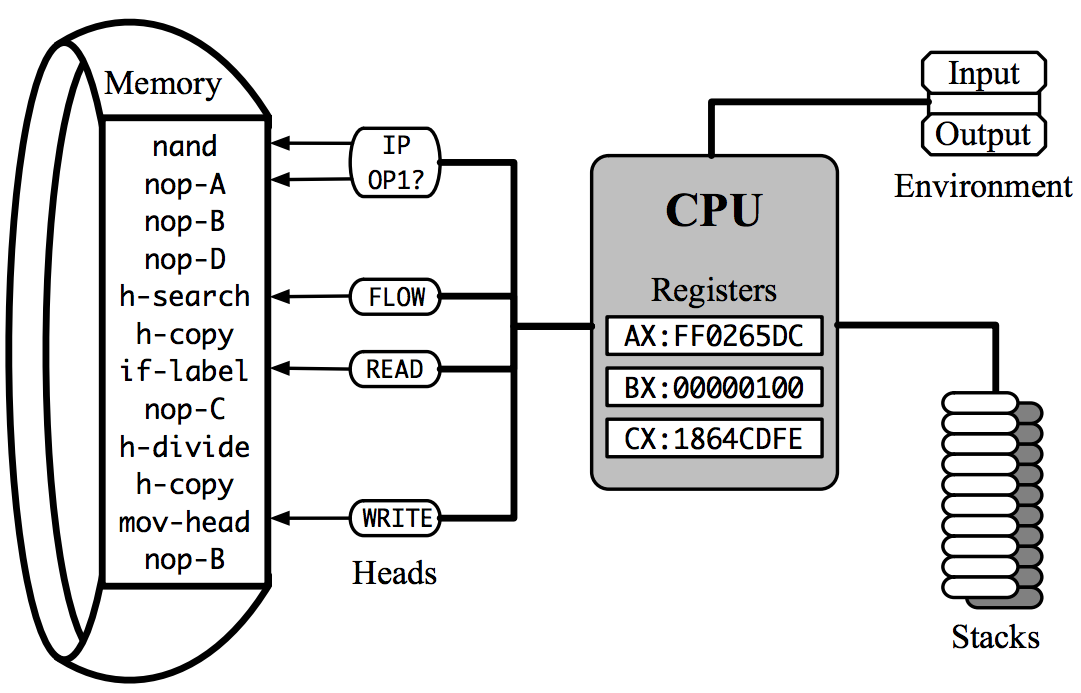
\includegraphics[width=\columnwidth]{imgs/virtual_hardware}
  \caption{\small Evaluation of Avida genome program instructions by virtual hardware, reproduced from \citep{Ofria:2009avida}.}
  \label{fig:vhardware}
\end{figure}


\noindent
Digital Organisms in Avida compete to acquire resources and replicate within limited space in a finite population.
Each organism is defined by a linear sequence of program instructions (\textit{i.e.} its genotype) and a set of virtual hardware. The instruction set in Avida is Turing Complete and syntactically robust -- any ordering of instructions is syntactically valid, though not always useful. The instruction set includes operations for basic computations, execution flow control, input and output, and self-replication. An organism's virtual hardware (depicted in Figure \ref{fig:vhardware}) consists of components such as a central processing unit (CPU), registers for computation, buffers for input and output, and memory stacks.

Organisms in Avida replicate asexually by allocating memory for their offspring, copying their genome instruction-by-instruction, and then dividing. However, copy and divide operations have imperfect fidelity and can result in mutated offspring. Organisms can influence their replication speed by improving their metabolic rate. An organism's metabolic rate determines the speed at which it executes instructions in its genome; a higher metabolic rate allows an organism to execute its genome faster, and thus, allows the organism to copy itself faster. Initially, an organism's metabolic rate set proportional to its length, so as to prevent intrinsic disadvantage from increased copy loop duration for long genomes. However, an organism's metabolic rate can be improved when it completes a particular task, such as a mathematical computation. In this way, we can differentially reward the performance of computational tasks.

When an organism finishes replicating, its offspring is placed in a random location elsewhere in the population, replacing that location's previous occupant.
Thus, improving the efficiency of self-replication or performing rewarded computational tasks are both advantageous in the competition for space in Avida. The combination of competition and heritable variation due to imperfect copy and divide operations results in evolution by natural selection in Avida \citep{pennock2007models}.

\begin{figure}[!ht]
\centering
% https://docs.google.com/presentation/d/109vfeK_lHSsE0q7Iz7tzl9sDxnP8jyOF2gJ-v85pgL8/edit?usp=sharing
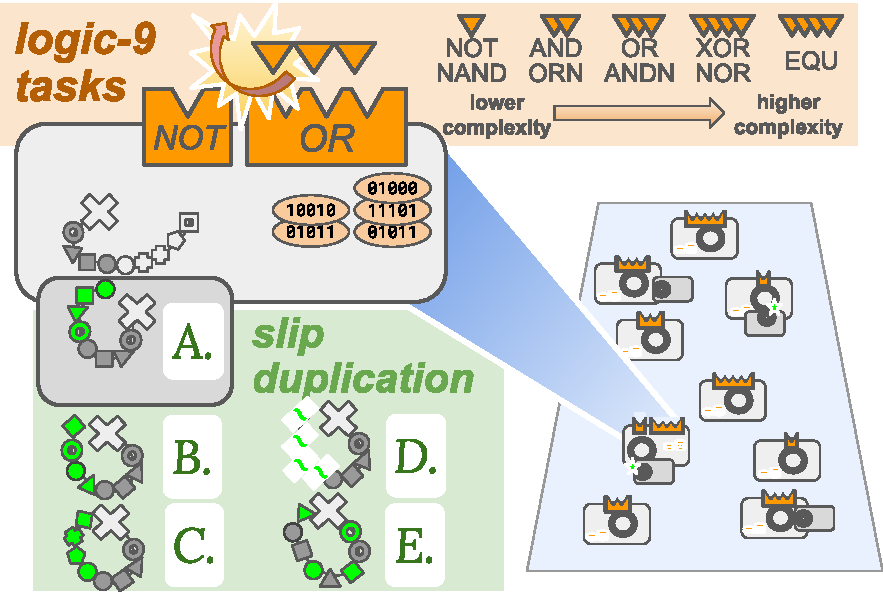
\includegraphics[width=\linewidth]{imgs/GeneDupeOps.pdf}
\caption{%
\textbf{Genome replication and phenotypic traits in Avida.}
\footnotesize
Self-replicating computer programs serve as digital model organisms.
Organisms comprise virtual stacks and registers used to store binary values and pointers within a circular genome of program instructions used to track instruction execution and copying.
Organisms compete to survive and reproduce within a limited-capacity population.
Replication activity can be accelerated by carrying out available ``logic-9'' input/output tasks.
% @AML: Readers might not know what is meant by "gates"; would lean toward "instructions" instead.
These tasks vary in complexity with respect to the number of NAND instructions required to perform them.
An organism's logic-9 ``phenotype'' arises from the expression of its genetic code.
Genetic code copied from parent to offspring may be subject to point mutations, which change the individual instruction values, and slip mutations, which introduce or remove many instructions all at once.
Reported experiments compare five alternate variants of slip mutation:
A) \textit{Slip-duplicate}, an exact duplication is inserted adjacent to the target segment;
B) \textit{Slip-scramble}, shuffled duplication is inserted directly after the target segment;
C) \textit{Slip-random}, random instructions are inserted directly after the target segment;
D) \textit{Slip-NOP}, neutral nop-X instructions are inserted directly after the target segment; and
E) \textit{Slip-scatter}, randomly-drawn instructions are inserted at random throughout the genome.
}
\label{fig:slip_mut_variants}
\end{figure}

\medskip
\noindent
\textbf{Mutation events in Avida} come in four types: substitution, insertion, deletion, or slip. Rates of occurance for each may be independently configured.

\textit{Copy mutations} occur when a copy instruction errs.
If it is a \textit{substitution} error, a random instruction is written to the copy location instead of the intended instruction.
If it is an \textit{insertion}, a random extra instruction is copied along with the intended instruction.
If it is a \textit{deletion}, the copy instruction fails to write any instruction at all.

\textit{Divide mutations} act on an organism's offspring during division.
When a divide \textit{insertion} mutation occurs, a randomly-chosen instruction is inserted at random into the offspring's genome, increasing the size of the offspring's genome by one.
When a divide \textit{deletion} mutation occurs, a random instruction in the offspring's genome is removed, decreasing the size of the offspring's genome by one.

For the purposes of this study, we implemented a new type of divide mutations: \textit{Slip mutations}.
This type of mutation acts analogously to gene duplications and deletions.
When a slip mutation occurs, two sites in the offspring genome are randomly selected, defining the target segment for the operation. If the first site is upstream of the second, the slip mutation results in an insertion --- as if the organism's replication machinery had slipped backward during replication and recopied a segment. If the second site is upstream of the first, the slip mutation results in a deletion --- as if the organism's replication machinery slipped forward during replication, skipping over a genetic segment. As implemented, slip-insertions and slip-deletions occur with equal probability; thus, absent selection, this mutational process do not introduce an inherent bias on genome length.

%ELD: If you're going to list the names of all the mutations, you might want to explain what exactly they each do that makes them different from each other.
Across trials, we assess five variants of slip mutations: slip-duplicate, slip-scramble, slip-random, slip-NOP, and slip-scatter. When a slip mutation results in a deletion, in all but the slip-scatter variant, the target segment is deleted. Rather than deleting the target segment, the slip-scatter mutation operator distributes a number of single-instruction deletions equal to the length of the target segment uniformly throughout the genome. When a slip mutation results in an insertion, a number of instructions equal to the length of the target segment is inserted into the genome; however, depending on the particular slip mutation operator, which instructions are inserted and where the insertions take place may be different. Figure \ref{fig:slip_mut_variants} provides description and examples of how each slip mutation operator handles insertions. % MJW: The rest of this paragraph is repetitive with the information about the slip mutations found withing the Treatments subsection.  I am therefore commenting it out.  Also, because this now is very short (it originally started with "When a slip mutation results in an insertion"), I am combining that into the previous paragraph.
%The slip-duplicate operator is capable of maintaining both the content and structure (\textit{i.e.} the ordering) of duplicated instruction sequences. The slip-scramble operator maintains the content but not the structure of duplicated sequences. The slip-random operator maintains neither the content nor the structure of duplicated sequences. The slip-NOP operator only inserts blank `genetic tape', increasing genome size without inserting anything meaningful. Instead of inserting duplicated code, the slip-scatter operator makes a number of random insertions in random locations in the genome equal to the length of the would-be duplicated code.

\subsection{Experimental Design}

Across all experiments, we rewarded the performance of nine Boolean logic functions: NOT, NAND, OR-NOT, AND, OR, AND-NOT, NOR, XOR, and EQUALS.
(Detailed description of this ``Logic-9'' task set can be found in \citet{lenski2003evolutionary}).
Rewards for these functions were identical and consistent for the duration of the experiment.

In , we evaluated the number of unique computational tasks it could perform, resulting in a \textit{phenotypic match score} that indicates how well the organism is adapted to the static environment. Phenotypic match scores in the static environment range from a minimum of 0 (\textit{i.e.} the organism performs no tasks) to a maximum of 9 (\textit{i.e.} the organism performs all 9 tasks). %We describe phenotypic match scores for the static environment, $Score_s$, mathematically in
Equation \ref{Equ:static_phen_match_score} describes the static match score ($Score_s$), where $P$ is a phenotype and $P_s$ represents the set of tasks phenotype $P$ performs in the static environment.

\begin{equation}
Score_s(P) = |P_{s}|
\label{Equ:static_phen_match_score}
\end{equation}

\footnote{An update in Avida is equal to the amount of time it takes for the average organism to execute 30 instructions; see \citep{Ofria:2009avida} for further detail.}

% Color Definitions (for treatments table)
\newcommand\baselineratecolor{\cellcolor[HTML]{c9daf8}}
\newcommand\nonecolor{\cellcolor[HTML]{666666}}
\newcommand\slipdupcolor{\cellcolor[HTML]{4a86e8}}
\newcommand\slipscramcolor{\cellcolor[HTML]{8e7cc3}}
\newcommand\sliprandcolor{\cellcolor[HTML]{93c47d}}
\newcommand\slipnopcolor{\cellcolor[HTML]{ffd966}}
\newcommand\slipscattercolor{\cellcolor[HTML]{e06666}}
\newcommand\highmutcolor{\cellcolor[HTML]{ff9900}}

\begin{table*}[!ht]
  \centering
  \begin{tblr}{| c | c | c | c | c | c | c | c |}
    \hline
    \SetCell[r=2]{c} Treatment & \SetCell[c=2]{c} Slip Mutation & & \SetCell[r=2]{c} Substitution rate \\ per copy & \SetCell[r=2]{c} Insertion \\ and deletion rate \\ per copy & \SetCell[r=2]{c} Insertion and \\ deletion rate \\ per divide \\
    \cline{2-3}
    & Operator & Rate \\ per divide & & & \\
    \hline
    Baseline            & \nonecolor & \nonecolor & 0.0025 \baselineratecolor & \nonecolor & 0.05 \baselineratecolor  \\
    \hline
    Slip-duplicate      & Slip-duplicate \slipdupcolor & 0.05 \slipdupcolor   & 0.0025 \baselineratecolor & \nonecolor   & 0.05 \baselineratecolor  \\
    \hline
    Slip-scramble       & Slip-scramble \slipscramcolor & 0.05 \slipscramcolor    & 0.0025 \baselineratecolor & \nonecolor & 0.05 \baselineratecolor  \\
    \hline
    Slip-random         & Slip-random \sliprandcolor & 0.05 \sliprandcolor   & 0.0025 \baselineratecolor & \nonecolor & 0.05 \baselineratecolor  \\
    \hline
    Slip-NOP            & Slip-NOP \slipnopcolor  & 0.05 \slipnopcolor   & 0.0025 \baselineratecolor & \nonecolor & 0.05 \baselineratecolor  \\
    \hline
    Slip-scatter        & Slip-scatter \slipscattercolor & 0.05 \slipscattercolor & 0.0025 \baselineratecolor & \nonecolor & 0.05 \baselineratecolor  \\
    \hline
    High mutation rate  & \nonecolor & \nonecolor & 0.0025 \baselineratecolor & 0.0075 \highmutcolor & 0.05 \baselineratecolor \\
    \hline
  \end{tblr}
  \caption{\small Differences in mutation operators and rates among the seven treatments.}
  \label{table:treatments}
\end{table*}

Our experiment consisted of seven treatments: one baseline treatment and six experimental treatments. Treatments differed only in the available mutation operators and the rates at which those operators were applied. Each treatment was designed to tease apart why gene duplications promote evolvability. Table \ref{table:treatments} provides details about each treatment.

% Baseline treatment
The \textbf{baseline treatment} was used as a control; we used the results from this treatment as a baseline for evolvability with which we compared the results from all other experimental treatments. Mutation rates in the baseline treatment have been shown to facilitate both the evolution of complex boolean logic tasks, such as EQUALS, and the evolution of task regulation in Avida \citep{lenski2003evolutionary, Lalejini:2016plasticity}

% Slip-duplicate treatment
The \textbf{slip-duplicate treatment} allowed for mutation events that resulted in full code duplications via the slip-duplicate mutation operator. Duplications in this treatment preserved both the content and the structure of duplicated code. This allowed us to answer the following question: how important is it that gene duplications can exactly duplicate sequences in a genome in both content \textit{and} structure?

% Slip-scramble treatment
The \textbf{slip-scramble treatment} allowed for mutation events (via the slip-scramble operator) that resulted in code duplications where the content of the duplicated code was preserved, but the structure of the duplicated code was not preserved. This, when compared with the slip-duplicate treatment, allowed us to answer the following question: is it that the duplication of particular instructions is important, regardless of their arrangement?

% Slip-random treatment
The \textbf{slip-random treatment} allowed us to answer the following question: is it the case that gene duplications promote evolvability because they result in the insertion of large, clustered mutations, regardless of what those mutations may be? The slip-random treatment (via the slip-random mutation operator) allowed for mutation events that could insert large, contiguous clusters of random instructions; one could also think of these mutations as maximally noisy duplications where neither the content or structure of the duplicated code is preserved.

% Slip-NOP treatment
The \textbf{slip-NOP treatment} allowed for mutations capable of inserting contiguous segments of blank `genetic tape' (via the slip-NOP mutation operator) in the form of no operation instructions. This allowed us to answer the following question: how important is it that gene duplications provide evolution with an easy technique for increasing genome size?

% Slip-scatter treatment
The \textbf{slip-scatter treatment} helped us to tease apart whether or not gene duplications promote evolvability because they inflate the effective mutation rate, generating increased amounts of genetic variation. This treatment allowed for mutations that, when triggered, could insert many random instructions into random locations in a genome (via the slip-scatter mutation operator).

% High mutation rate treatment
The \textbf{high mutation rate treatment} served a similar purpose to the slip-scatter treatment. However, instead of single mutation events (slip-scatter mutations) causing the insertion of many random instructions, we elevated the rates at which the copy instruction makes a random insertion or random deletion to result in approximately the same number of mutations per divide as in any treatment that includes a slip mutation operator. This allowed us to evaluate the importance of having an increased mutation rate due to large-scale, single-event mutations versus having a higher copy mutation rate.

% Long genome treatment
To better discern the role in facilitating evolution of larger genome size caused by gene duplication, we performed an additional treatment: the \textbf{long-genome baseline treatment}.
Genomes in this treatment operated identically to the baseline treatment above, except that they were 1,000 sites long instead of 100 sites long.
We chose this size as it was near the upper bound of the largest genome sizes that we observed in the slip-duplication treatment experiments.

In all experiments, organisms were limited to a minimum genome size (\textit{i.e.} instruction sequence length) of 100\footnote{
In exploratory experiments, we found that, without enforcing a minimum genome size, slip mutations caused many lineages to quickly shrink in genome size because of inherent selection pressure for smaller genome size. Organisms became fast replicators but were then trapped on a local fitness optima, unable to evolve to perform complex computational tasks.
}.
We limited the population size to 3600 and seeded each experiment with an ancestral genotype capable of self-replication, but no logic-9 task.
In both the static environment and simple changing environments, populations evolved for 200000 updates.
We ran TODO trials of each treatment.

\subsection{Statistical Methods}

To determine if any of the treatments was significant within a set, we performed a Kruskal-Wallis test, applying a Bonferroni correction (for an earlier experimental design incorporating two additional surveyed environments) to keep the experiment-wise $\alpha$ = 0.05.
For an environment in which the Kruskal-Wallis test was significant, we performed Mann-Whitney U tests for each experimental treatment against the control, and applied a Bonferroni correction for the six such tests within each environment.

\subsubsection{Digital Organism Evaluation}
At the end of each trial, we extracted the final dominant (most abundant) genotype in the population, and we traced back that genotype's full ancestral lineage.
We calculated the phenotypic match score for each final dominant organism and all of their ancestors.

TODO discuss tracking mutations back along lineages

\subsection{Software and Data Availability} \label{sec:materials}

Supporting software and executable notebooks for this work are available via Zenodo at TODO \citep{TODO} and on GitHub at \url{https://github.com/chaynes2019/AvidaGeneDupe/}.
Simulation data is archived via the Open Science Framework at \url{https://osf.io/j5s4h/} \citep{foster2017open}.

This project benefited significantly from a large number of open-source scientific software projects \citep{2020SciPy-NMeth,harris2020array,reback2020pandas,mckinney-proc-scipy-2010,waskom2021seaborn,hunter2007matplotlib,moreno2023teeplot,r_core_team_r:_2015}.
